\chapter{CoAP library module}

\section{Architectuur}

\subsection{Functionaliteit}

Hier komt de functionaliteit van de CoAP library.\\

Een van de belangrijkste aspecten bij deze masterproef is een minimale belasting te realiseren voor de sensoren, dit is immers de reden voor de ontwikkeling van CoAP. Opgehaalde waarden zullen dan ook in de databank worden opgeslagen met een geldigheidswaarde, wanneer een waarde nog geldig is, wordt de waarde uit de databank gehaald en wordt het embedded device niet opnieuw bevraagd. Slechts wanneer de waarde niet meer geldig is, wordt het embedded device aangesproken.\\

\subsection{Content-type in de databank}

Wanneer data ontvangen wordt, moet deze opgeslagen worden in de databank. Er moet dan ook een tabel voorzien worden in de databank met de nodige velden, het content-type in de databank:

\begin{wrapfigure}{r}{0.3\textwidth}
\vspace{10pt}
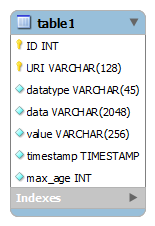
\includegraphics[width=0.3\textwidth]{fig/contentTypeDatabank}
\vspace{-35pt}
\caption{Content-type in databank}
\vspace{-10pt}
\end{wrapfigure}
\paragraph{}
\vspace*{-\parskip}

\begin{itemize}
\item Een ID van de resource,
\item de URI van het embedded device,
\item het datatype van de ontvangen waarde (XML, JSON, plain text, etc),
\item de effectieve data (originele, raw input),
\item de verwerkte data,
\item een timestamp die het tijdstip van opvragen aanduidt,
\item waarde om de geldigheid te controleren (max age).
\end{itemize}
